\section{RiverSwim MDP}

Now you will implement value iteration and policy iteration for the RiverSwim environment (see picture below\footnote{Figure copied from \href{https://proceedings.neurips.cc/paper/2013/hash/6a5889bb0190d0211a991f47bb19a777-Abstract.html}{(Osband \& Van Roy, 2013)}.}) of \href{https://www.sciencedirect.com/science/article/pii/S0022000008000767}{(Strehl \& Littman, 2008)}.

\begin{figure}[h]
  \centering
  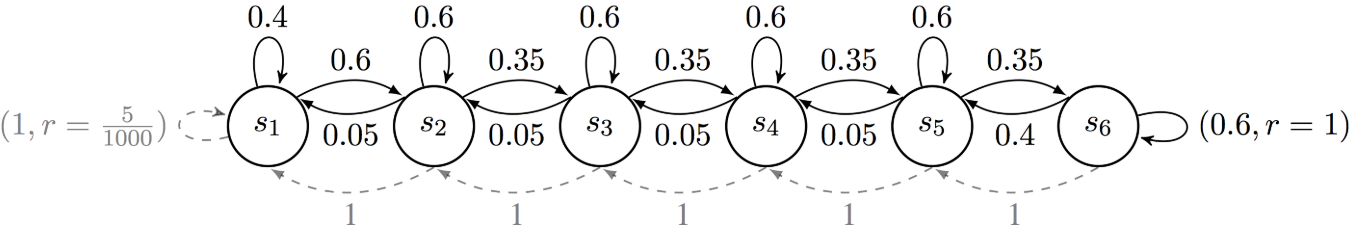
\includegraphics[width=\linewidth]{images/RiverSwim.png}
  \caption{The RiverSwim MDP where dashed and solid arrows represent transitions for the \textsc{LEFT} and \textsc{RIGHT} actions, respectively. The assignment uses a modified, customizable version of what is shown above where there are three different strengths (\textsc{WEAK}, \textsc{MEDIUM}, or \textsc{STRONG}) of the current (transition probabilities for being pushed back or successfully swimming \textsc{RIGHT}).}
  \label{fig:riverswim}
\end{figure}

\textit{Note:} Run \texttt{python submission.py} for RiverSwim with a discount factor $\gamma = 0.99$ and a \textsc{weak} current, You can use this to verify your implementation. For grading purposes, we shall test your implementation against base and hidden test cases in \texttt{grader.py}.

\begin{enumerate}[(a)]

  \item \points{1a}

Read through \texttt{submission.py} and implement \texttt{bellman\_backup}. Return the value associated with a single Bellman backup performed for an input state-action pair.

\textbf{Important}: please use the version presented in the class and not any variants of it!

  \item \points{1b}

Implement \texttt{policy\_evaluation} in  \texttt{submission.py}. Return the optimal value function.

  \item \points{1c}

Implement \texttt{policy\_improvement} in  \texttt{submission.py}. Return the optimal policy.

  \item \points{1d}

Implement \texttt{policy\_iteration} in \texttt{submission.py}. Return the optimal value function and the optimal policy.

  \item \points{1e}

Implement \texttt{value\_iteration} in \texttt{submission.py}. Return the optimal value function and the optimal policy.

  \input{01-riverswim/06-currents}

\end{enumerate}